\documentclass[letterpaper,12pt]{article}
\usepackage{array}
\usepackage{threeparttable}
\usepackage{geometry}
\geometry{letterpaper,tmargin=1in,bmargin=1in,lmargin=1.25in,rmargin=1.25in}
\usepackage{fancyhdr,lastpage}
\pagestyle{fancy}
\lhead{}
\chead{}
\rhead{}
\lfoot{}
\cfoot{}
\rfoot{\footnotesize\textsl{Page \thepage\ of \pageref{LastPage}}}
\renewcommand\headrulewidth{0pt}
\renewcommand\footrulewidth{0pt}
\usepackage[format=hang,font=normalsize,labelfont=bf]{caption}
\usepackage{listings}
\usepackage{color}
\definecolor{dkgreen}{rgb}{0,0.6,0}
\definecolor{gray}{rgb}{0.5,0.5,0.5}
\definecolor{mauve}{rgb}{0.58,0,0.82}
\lstset{ %
  language=R,                     % the language of the code
  basicstyle=\footnotesize,       % the size of the fonts that are used for the code
  numbers=left,                   % where to put the line-numbers
  numberstyle=\tiny\color{gray},  % the style that is used for the line-numbers
  stepnumber=1,                   % the step between two line-numbers. If it's 1, each line
  numbersep=5pt,                  % how far the line-numbers are from the code
  backgroundcolor=\color{white},  % choose the background color. You must add \usepackage{color}
  showspaces=false,               % show spaces adding particular underscores
  showstringspaces=false,         % underline spaces within strings
  showtabs=false,                 % show tabs within strings adding particular underscores
  frame=single,                   % adds a frame around the code
  rulecolor=\color{black},        % if not set, the frame-color may be changed on line-breaks within not-black text (e.g. commens (green here))
  tabsize=2,                      % sets default tabsize to 2 spaces
  captionpos=b,                   % sets the caption-position to bottom
  breaklines=true,                % sets automatic line breaking
  breakatwhitespace=false,        % sets if automatic breaks should only happen at whitespace
  title=\lstname,                 % show the filename of files included with \lstinputlisting;
  keywordstyle=\color{blue},      % keyword style
  commentstyle=\color{dkgreen},   % comment style
  stringstyle=\color{mauve},      % string literal style
  escapeinside={\%*}{*)},         % if you want to add a comment within your code
  morekeywords={*,...}            % if you want to add more keywords to the set
}
\usepackage{amsmath}
\usepackage{amssymb}
\usepackage{amsthm}
\usepackage{harvard}
\usepackage{setspace}
\usepackage{float,color}
\usepackage[pdftex]{graphicx}
\usepackage{hyperref}
\hypersetup{colorlinks,linkcolor=red,urlcolor=blue}
\theoremstyle{definition}
\newtheorem{theorem}{Theorem}
\newtheorem{acknowledgement}[theorem]{Acknowledgement}
\newtheorem{algorithm}[theorem]{Algorithm}
\newtheorem{axiom}[theorem]{Axiom}
\newtheorem{case}[theorem]{Case}
\newtheorem{claim}[theorem]{Claim}
\newtheorem{conclusion}[theorem]{Conclusion}
\newtheorem{condition}[theorem]{Condition}
\newtheorem{conjecture}[theorem]{Conjecture}
\newtheorem{corollary}[theorem]{Corollary}
\newtheorem{criterion}[theorem]{Criterion}
\newtheorem{definition}[theorem]{Definition}
\newtheorem{derivation}{Derivation} % Number derivations on their own
\newtheorem{example}[theorem]{Example}
\newtheorem{exercise}[theorem]{Exercise}
\newtheorem{lemma}[theorem]{Lemma}
\newtheorem{notation}[theorem]{Notation}
\newtheorem{problem}[theorem]{Problem}
\newtheorem{proposition}{Proposition} % Number propositions on their own
\newtheorem{remark}[theorem]{Remark}
\newtheorem{solution}[theorem]{Solution}
\newtheorem{summary}[theorem]{Summary}
%\numberwithin{equation}{section}
\bibliographystyle{aer}
\newcommand\ve{\varepsilon}
\newcommand\boldline{\arrayrulewidth{1pt}\hline}


\begin{document}

\begin{flushleft}
  \textbf{\large{Problem Set \#3}} \\
  MACS 30100, Dr. Evans \\
  Cheng Yee Lim
\end{flushleft}

\vspace{5mm}

\noindent\textbf{Problem 1}\\
\textbf{Part (a).}
\begin{figure}[htb]\centering\captionsetup{width=4.0in}
  \caption{\textbf{Normed Histogram of Percentages of income}}\label{FigExample}
  \fbox{\resizebox{6.0in}{4.0in}{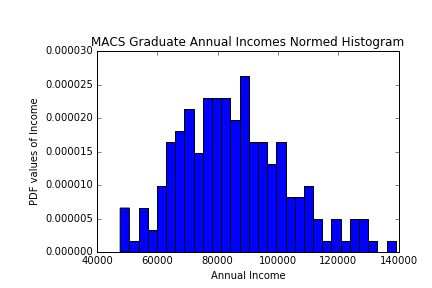
\includegraphics{images/1a.png}}}
\end{figure}

\pagebreak
\textbf{Part (b).} \\
\begin{figure}[htb]\centering\captionsetup{width=4.0in}
  \caption{\textbf{Normed histogram of Annual Incomes of MACSS Graduates and the LogNormal PDF}}\label{FigExample}
  \fbox{\resizebox{6.0in}{4.0in}{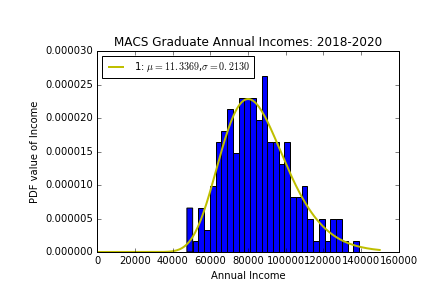
\includegraphics{images/1b.png}}}
\end{figure}

\flushleft 
The estimated $\mu_{GMM_1}$ is 11.3369 and the estimated $\sigma\_{GMM_1}$ is 0.2130.\\
The GMM criterion function is $3.93977\times10^{-13}$.\\
Two data moments, $mu$ and $sigma$, are 85276.824 and 17992.542.
Two model moments, $mu$ and $sigma$, are 85276.795 and 17992.533.
The data and model moments are highly similar, in fact the mean data and model moment are identical to 5 significant factors and the standard deviation moment are identical to 6 significant factors. The highly similar data and model moments show that the GMM estimation was a good estimation. 

\pagebreak

\textbf{Part (c).} \\
\begin{figure}[htb]\centering\captionsetup{width=4.0in}
  \caption{\textbf{Normed Histogram of MACSS Students Annual Income and Log PDFs}}\label{FigExample}
  \fbox{\resizebox{6.0in}{4.0in}{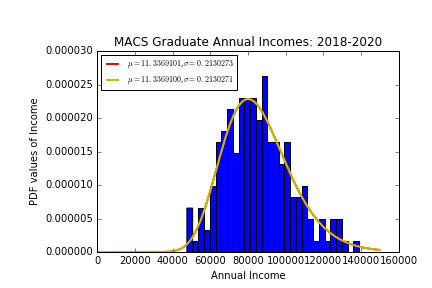
\includegraphics{images/1c.png}}}
\end{figure}
\flushleft 
The GMM estimates for $\mu$ and $\sigma$ are 11.3369101002 and 0.213027153205.\\ 
The GMM criterion function is $2.2371736191\times10^{-10}$.\\
Two data moments, $mu$ and $sigma$, are 85276.824 and 17992.542.\\
Two model moments, $mu$ and $sigma$, are 85276.804 and 17992.545.\\
Expectedly, the results of the two step variance covariance weights matrix GMM estimation are highly similar to the data moments. However, since the estimation in part (b) was already close to perfect, a marked improvement could not be seen comparing part (c) to (b) as both estimations were good estimations. 


\pagebreak
\textbf{Part (d).} \\
\flushleft 
\begin{figure}[htb]\centering\captionsetup{width=4.0in}
  \caption{\textbf{Normed histogram of Annual Incomes of MACSS Graduates and the three moment LogNormal PDF}}\label{FigExample}
  \fbox{\resizebox{6.0in}{4.0in}{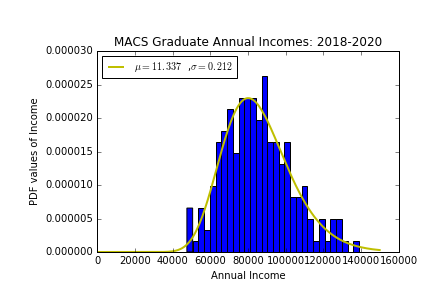
\includegraphics{images/1d.png}}}
\end{figure}
\flushleft 
The estimated $\mu$ is 11.337 and the estimated $\sigma$ is 0.212.\\
The GMM criterion function is 0.238.\\
The three data moments are (0.3, 0.5, 0.2).\\
The three model moments are (0.2993, 0.4981, 0.199663).\\
Comparing the three data and model moments, we can see that the GMM estimated parameters gave very close estimations to the actual data. Thus, this was a good estimation as well. 

\pagebreak

\textbf{Part (e).} \\
\begin{figure}[htb]\centering\captionsetup{width=4.0in}
  \caption{\textbf{Normed histogram of Annual Incomes of MACSS Graduates and the three moment LogNormal PDF}}\label{FigExample}
  \fbox{\resizebox{6.0in}{4.0in}{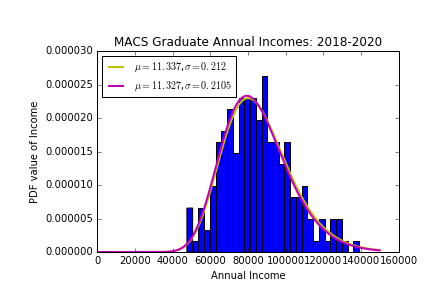
\includegraphics{images/1e.png}}}
\end{figure}
\flushleft

The estimated $\mu$ is 11.327 and the estimated $\sigma$ is 0.2105.\\
The value of the GMM criterion is $2.93379037473 \times 10^{-5}$. \\
The three data moments are (0.3, 0.5, 0.2).\\
The three model moments are (0.3141, 0.4972, 0.1862).\\
In part (e), I used the inverse of the variance covariance matrix to obtain the weighting matrix and used the weighting matrix in the GMM estimation of the mean and standard deviation. The approximation in this case fared less well than part (d), where an identity matrix was used as the weighting matrix. There were larger deviations in data and model moments, for all three moments, when income was lesser than \$75,000, income was between \$75,000 and \$100,000, and when income was more than \$100,000. Thus, the estimation in part (e) fared worse in all three moments when compared to part (d). 

\pagebreak

\textbf{Part (f).}
\flushleft
Part (b), (c) and (d) fits the data equally well. The data and model moments were almost identical in all parts (b), (c) and (d), especially when rounded to 5 significant factors. The lognormal PDF graph captured the mean and the standard deviation of the data well. The PDF graph is especially good in fitting the data for income less than \$40,000, but less great in fitting the data for income more than \$120,000. Thus, if a fourth moment of more than \$125,000 was created, perhaps the GMM estimation with four moments could outdo the estimation in part (b) and (c). \\
\flushleft
\noindent\textbf{Problem 2}\\
\textbf{Part (a).} \\
\flushleft 
The estimates for the parameters of the model are as follows: \\
$\beta_0$ = 0.252, $\beta_1$ = 0.0129, $\beta_2$ = 0.401, $\beta_3$ = -0.010\\
The value of GMM criterion function at the estimated parameter values is 0.00182.

\end{document}
